% Graphic for TeX using PGF
% Title: /home/lluis/Escritorio/TFM/Informe/images/dcm_driver_flow.dia
% Creator: Dia v0.97.2
% CreationDate: Sat May 28 14:20:42 2016
% For: lluis
% \usepackage{tikz}
% The following commands are not supported in PSTricks at present
% We define them conditionally, so when they are implemented,
% this pgf file will use them.
\ifx\du\undefined
  \newlength{\du}
\fi
\setlength{\du}{15\unitlength}
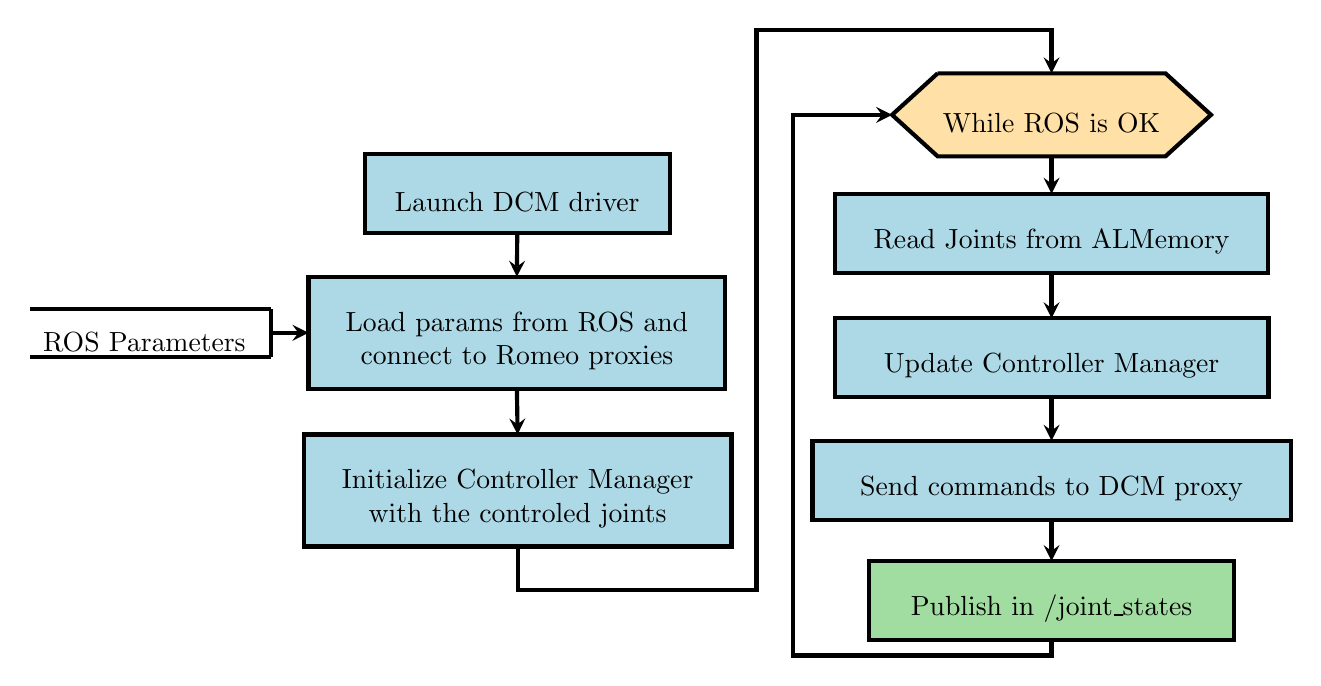
\begin{tikzpicture}
\pgftransformxscale{1.000000}
\pgftransformyscale{-1.000000}
\definecolor{dialinecolor}{rgb}{0.000000, 0.000000, 0.000000}
\pgfsetstrokecolor{dialinecolor}
\definecolor{dialinecolor}{rgb}{1.000000, 1.000000, 1.000000}
\pgfsetfillcolor{dialinecolor}
\definecolor{dialinecolor}{rgb}{0.678431, 0.847059, 0.901961}
\pgfsetfillcolor{dialinecolor}
\fill (17.445000\du,4.450000\du)--(17.445000\du,6.350000\du)--(24.795124\du,6.350000\du)--(24.795124\du,4.450000\du)--cycle;
\pgfsetlinewidth{0.100000\du}
\pgfsetdash{}{0pt}
\pgfsetdash{}{0pt}
\pgfsetmiterjoin
\definecolor{dialinecolor}{rgb}{0.000000, 0.000000, 0.000000}
\pgfsetstrokecolor{dialinecolor}
\draw (17.445000\du,4.450000\du)--(17.445000\du,6.350000\du)--(24.795124\du,6.350000\du)--(24.795124\du,4.450000\du)--cycle;
% setfont left to latex
\definecolor{dialinecolor}{rgb}{0.000000, 0.000000, 0.000000}
\pgfsetstrokecolor{dialinecolor}
\node at (21.120062\du,5.595000\du){Launch DCM driver};
\definecolor{dialinecolor}{rgb}{0.678431, 0.847059, 0.901961}
\pgfsetfillcolor{dialinecolor}
\fill (15.976200\du,11.200000\du)--(15.976200\du,13.900000\du)--(26.281575\du,13.900000\du)--(26.281575\du,11.200000\du)--cycle;
\pgfsetlinewidth{0.100000\du}
\pgfsetdash{}{0pt}
\pgfsetdash{}{0pt}
\pgfsetmiterjoin
\definecolor{dialinecolor}{rgb}{0.000000, 0.000000, 0.000000}
\pgfsetstrokecolor{dialinecolor}
\draw (15.976200\du,11.200000\du)--(15.976200\du,13.900000\du)--(26.281575\du,13.900000\du)--(26.281575\du,11.200000\du)--cycle;
% setfont left to latex
\definecolor{dialinecolor}{rgb}{0.000000, 0.000000, 0.000000}
\pgfsetstrokecolor{dialinecolor}
\node at (21.128888\du,12.345000\du){Initialize Controller Manager};
% setfont left to latex
\definecolor{dialinecolor}{rgb}{0.000000, 0.000000, 0.000000}
\pgfsetstrokecolor{dialinecolor}
\node at (21.128888\du,13.145000\du){with the controled joints};
\definecolor{dialinecolor}{rgb}{0.678431, 0.847059, 0.901961}
\pgfsetfillcolor{dialinecolor}
\fill (16.090000\du,7.400000\du)--(16.090000\du,10.100000\du)--(26.132975\du,10.100000\du)--(26.132975\du,7.400000\du)--cycle;
\pgfsetlinewidth{0.100000\du}
\pgfsetdash{}{0pt}
\pgfsetdash{}{0pt}
\pgfsetmiterjoin
\definecolor{dialinecolor}{rgb}{0.000000, 0.000000, 0.000000}
\pgfsetstrokecolor{dialinecolor}
\draw (16.090000\du,7.400000\du)--(16.090000\du,10.100000\du)--(26.132975\du,10.100000\du)--(26.132975\du,7.400000\du)--cycle;
% setfont left to latex
\definecolor{dialinecolor}{rgb}{0.000000, 0.000000, 0.000000}
\pgfsetstrokecolor{dialinecolor}
\node at (21.111488\du,8.545000\du){Load params from ROS and};
% setfont left to latex
\definecolor{dialinecolor}{rgb}{0.000000, 0.000000, 0.000000}
\pgfsetstrokecolor{dialinecolor}
\node at (21.111488\du,9.345000\du){connect to Romeo proxies};
\pgfsetlinewidth{0.100000\du}
\pgfsetdash{}{0pt}
\pgfsetdash{}{0pt}
\pgfsetbuttcap
\pgfsetmiterjoin
\pgfsetlinewidth{0.100000\du}
\pgfsetbuttcap
\pgfsetmiterjoin
\pgfsetdash{}{0pt}
\definecolor{dialinecolor}{rgb}{1.000000, 0.878431, 0.650980}
\pgfsetfillcolor{dialinecolor}
\pgfpathmoveto{\pgfpoint{31.247538\du}{2.500000\du}}
\pgfpathlineto{\pgfpoint{36.735038\du}{2.500000\du}}
\pgfpathlineto{\pgfpoint{37.832538\du}{3.500000\du}}
\pgfpathlineto{\pgfpoint{36.735038\du}{4.500000\du}}
\pgfpathlineto{\pgfpoint{31.247538\du}{4.500000\du}}
\pgfpathlineto{\pgfpoint{30.150038\du}{3.500000\du}}
\pgfpathlineto{\pgfpoint{31.247538\du}{2.500000\du}}
\pgfusepath{fill}
\definecolor{dialinecolor}{rgb}{0.000000, 0.000000, 0.000000}
\pgfsetstrokecolor{dialinecolor}
\pgfpathmoveto{\pgfpoint{31.247538\du}{2.500000\du}}
\pgfpathlineto{\pgfpoint{36.735038\du}{2.500000\du}}
\pgfpathlineto{\pgfpoint{37.832538\du}{3.500000\du}}
\pgfpathlineto{\pgfpoint{36.735038\du}{4.500000\du}}
\pgfpathlineto{\pgfpoint{31.247538\du}{4.500000\du}}
\pgfpathlineto{\pgfpoint{30.150038\du}{3.500000\du}}
\pgfpathlineto{\pgfpoint{31.247538\du}{2.500000\du}}
\pgfusepath{stroke}
% setfont left to latex
\definecolor{dialinecolor}{rgb}{0.000000, 0.000000, 0.000000}
\pgfsetstrokecolor{dialinecolor}
\node at (33.991288\du,3.700000\du){While ROS is OK};
\definecolor{dialinecolor}{rgb}{0.678431, 0.847059, 0.901961}
\pgfsetfillcolor{dialinecolor}
\fill (28.778607\du,5.400000\du)--(28.778607\du,7.300000\du)--(39.203968\du,7.300000\du)--(39.203968\du,5.400000\du)--cycle;
\pgfsetlinewidth{0.100000\du}
\pgfsetdash{}{0pt}
\pgfsetdash{}{0pt}
\pgfsetmiterjoin
\definecolor{dialinecolor}{rgb}{0.000000, 0.000000, 0.000000}
\pgfsetstrokecolor{dialinecolor}
\draw (28.778607\du,5.400000\du)--(28.778607\du,7.300000\du)--(39.203968\du,7.300000\du)--(39.203968\du,5.400000\du)--cycle;
% setfont left to latex
\definecolor{dialinecolor}{rgb}{0.000000, 0.000000, 0.000000}
\pgfsetstrokecolor{dialinecolor}
\node at (33.991288\du,6.545000\du){Read Joints from ALMemory};
\definecolor{dialinecolor}{rgb}{0.678431, 0.847059, 0.901961}
\pgfsetfillcolor{dialinecolor}
\fill (28.766960\du,8.400000\du)--(28.766960\du,10.300000\du)--(39.215616\du,10.300000\du)--(39.215616\du,8.400000\du)--cycle;
\pgfsetlinewidth{0.100000\du}
\pgfsetdash{}{0pt}
\pgfsetdash{}{0pt}
\pgfsetmiterjoin
\definecolor{dialinecolor}{rgb}{0.000000, 0.000000, 0.000000}
\pgfsetstrokecolor{dialinecolor}
\draw (28.766960\du,8.400000\du)--(28.766960\du,10.300000\du)--(39.215616\du,10.300000\du)--(39.215616\du,8.400000\du)--cycle;
% setfont left to latex
\definecolor{dialinecolor}{rgb}{0.000000, 0.000000, 0.000000}
\pgfsetstrokecolor{dialinecolor}
\node at (33.991288\du,9.545000\du){Update Controller Manager};
\definecolor{dialinecolor}{rgb}{0.678431, 0.847059, 0.901961}
\pgfsetfillcolor{dialinecolor}
\fill (28.231794\du,11.350000\du)--(28.231794\du,13.250000\du)--(39.750782\du,13.250000\du)--(39.750782\du,11.350000\du)--cycle;
\pgfsetlinewidth{0.100000\du}
\pgfsetdash{}{0pt}
\pgfsetdash{}{0pt}
\pgfsetmiterjoin
\definecolor{dialinecolor}{rgb}{0.000000, 0.000000, 0.000000}
\pgfsetstrokecolor{dialinecolor}
\draw (28.231794\du,11.350000\du)--(28.231794\du,13.250000\du)--(39.750782\du,13.250000\du)--(39.750782\du,11.350000\du)--cycle;
% setfont left to latex
\definecolor{dialinecolor}{rgb}{0.000000, 0.000000, 0.000000}
\pgfsetstrokecolor{dialinecolor}
\node at (33.991288\du,12.495000\du){Send commands to DCM proxy};
\definecolor{dialinecolor}{rgb}{0.631373, 0.862745, 0.631373}
\pgfsetfillcolor{dialinecolor}
\fill (29.591816\du,14.250000\du)--(29.591816\du,16.150000\du)--(38.390760\du,16.150000\du)--(38.390760\du,14.250000\du)--cycle;
\pgfsetlinewidth{0.100000\du}
\pgfsetdash{}{0pt}
\pgfsetdash{}{0pt}
\pgfsetmiterjoin
\definecolor{dialinecolor}{rgb}{0.000000, 0.000000, 0.000000}
\pgfsetstrokecolor{dialinecolor}
\draw (29.591816\du,14.250000\du)--(29.591816\du,16.150000\du)--(38.390760\du,16.150000\du)--(38.390760\du,14.250000\du)--cycle;
% setfont left to latex
\definecolor{dialinecolor}{rgb}{0.000000, 0.000000, 0.000000}
\pgfsetstrokecolor{dialinecolor}
\node at (33.991288\du,15.395000\du){Publish in /joint\_states};
\pgfsetlinewidth{0.100000\du}
\pgfsetdash{}{0pt}
\pgfsetdash{}{0pt}
\pgfsetmiterjoin
\pgfsetbuttcap
{
\definecolor{dialinecolor}{rgb}{0.000000, 0.000000, 0.000000}
\pgfsetfillcolor{dialinecolor}
% was here!!!
\pgfsetarrowsend{stealth}
{\pgfsetcornersarced{\pgfpoint{0.000000\du}{0.000000\du}}\definecolor{dialinecolor}{rgb}{0.000000, 0.000000, 0.000000}
\pgfsetstrokecolor{dialinecolor}
\draw (21.128900\du,13.900000\du)--(21.128900\du,14.950000\du)--(26.885078\du,14.950000\du)--(26.885078\du,1.450000\du)--(33.991288\du,1.450000\du)--(33.991288\du,2.500000\du);
}}
\pgfsetlinewidth{0.100000\du}
\pgfsetdash{}{0pt}
\pgfsetdash{}{0pt}
\pgfsetmiterjoin
\pgfsetbuttcap
{
\definecolor{dialinecolor}{rgb}{0.000000, 0.000000, 0.000000}
\pgfsetfillcolor{dialinecolor}
% was here!!!
\pgfsetarrowsend{stealth}
{\pgfsetcornersarced{\pgfpoint{0.000000\du}{0.000000\du}}\definecolor{dialinecolor}{rgb}{0.000000, 0.000000, 0.000000}
\pgfsetstrokecolor{dialinecolor}
\draw (33.991288\du,16.150000\du)--(33.991288\du,16.525544\du)--(27.768018\du,16.525544\du)--(27.768018\du,3.500000\du)--(30.150038\du,3.500000\du);
}}
\pgfsetlinewidth{0.100000\du}
\pgfsetdash{}{0pt}
\pgfsetdash{}{0pt}
\pgfsetbuttcap
{
\definecolor{dialinecolor}{rgb}{0.000000, 0.000000, 0.000000}
\pgfsetfillcolor{dialinecolor}
% was here!!!
\pgfsetarrowsend{stealth}
\definecolor{dialinecolor}{rgb}{0.000000, 0.000000, 0.000000}
\pgfsetstrokecolor{dialinecolor}
\draw (33.991288\du,4.500000\du)--(33.991288\du,5.400000\du);
}
\pgfsetlinewidth{0.100000\du}
\pgfsetdash{}{0pt}
\pgfsetdash{}{0pt}
\pgfsetbuttcap
{
\definecolor{dialinecolor}{rgb}{0.000000, 0.000000, 0.000000}
\pgfsetfillcolor{dialinecolor}
% was here!!!
\pgfsetarrowsend{stealth}
\definecolor{dialinecolor}{rgb}{0.000000, 0.000000, 0.000000}
\pgfsetstrokecolor{dialinecolor}
\draw (33.991288\du,7.300000\du)--(33.991288\du,8.400000\du);
}
\pgfsetlinewidth{0.100000\du}
\pgfsetdash{}{0pt}
\pgfsetdash{}{0pt}
\pgfsetbuttcap
{
\definecolor{dialinecolor}{rgb}{0.000000, 0.000000, 0.000000}
\pgfsetfillcolor{dialinecolor}
% was here!!!
\pgfsetarrowsend{stealth}
\definecolor{dialinecolor}{rgb}{0.000000, 0.000000, 0.000000}
\pgfsetstrokecolor{dialinecolor}
\draw (33.991288\du,10.300000\du)--(33.991288\du,11.350000\du);
}
\pgfsetlinewidth{0.100000\du}
\pgfsetdash{}{0pt}
\pgfsetdash{}{0pt}
\pgfsetbuttcap
{
\definecolor{dialinecolor}{rgb}{0.000000, 0.000000, 0.000000}
\pgfsetfillcolor{dialinecolor}
% was here!!!
\pgfsetarrowsend{stealth}
\definecolor{dialinecolor}{rgb}{0.000000, 0.000000, 0.000000}
\pgfsetstrokecolor{dialinecolor}
\draw (33.991288\du,13.250000\du)--(33.991288\du,14.250000\du);
}
\pgfsetlinewidth{0.100000\du}
\pgfsetdash{}{0pt}
\pgfsetdash{}{0pt}
\pgfsetbuttcap
{
\definecolor{dialinecolor}{rgb}{0.000000, 0.000000, 0.000000}
\pgfsetfillcolor{dialinecolor}
% was here!!!
\pgfsetarrowsend{stealth}
\definecolor{dialinecolor}{rgb}{0.000000, 0.000000, 0.000000}
\pgfsetstrokecolor{dialinecolor}
\draw (21.120100\du,6.350000\du)--(21.111500\du,7.400000\du);
}
\pgfsetlinewidth{0.100000\du}
\pgfsetdash{}{0pt}
\pgfsetdash{}{0pt}
\pgfsetbuttcap
{
\definecolor{dialinecolor}{rgb}{0.000000, 0.000000, 0.000000}
\pgfsetfillcolor{dialinecolor}
% was here!!!
\pgfsetarrowsend{stealth}
\definecolor{dialinecolor}{rgb}{0.000000, 0.000000, 0.000000}
\pgfsetstrokecolor{dialinecolor}
\draw (21.111500\du,10.100000\du)--(21.128900\du,11.200000\du);
}
\pgfsetlinewidth{0.100000\du}
\pgfsetdash{}{0pt}
\pgfsetdash{}{0pt}
\pgfsetbuttcap
\pgfsetmiterjoin
\pgfsetlinewidth{0.100000\du}
\pgfsetbuttcap
\pgfsetmiterjoin
\pgfsetdash{}{0pt}
\definecolor{dialinecolor}{rgb}{0.000000, 0.000000, 0.000000}
\pgfsetstrokecolor{dialinecolor}
\draw (15.189518\du,8.171050\du)--(15.189518\du,9.328945\du);
\pgfsetbuttcap
\pgfsetmiterjoin
\pgfsetdash{}{0pt}
\definecolor{dialinecolor}{rgb}{0.000000, 0.000000, 0.000000}
\pgfsetstrokecolor{dialinecolor}
\draw (15.189518\du,8.171050\du)--(9.376360\du,8.171050\du);
\pgfsetbuttcap
\pgfsetmiterjoin
\pgfsetdash{}{0pt}
\definecolor{dialinecolor}{rgb}{0.000000, 0.000000, 0.000000}
\pgfsetstrokecolor{dialinecolor}
\draw (15.189518\du,9.328945\du)--(9.376360\du,9.328945\du);
% setfont left to latex
\definecolor{dialinecolor}{rgb}{0.000000, 0.000000, 0.000000}
\pgfsetstrokecolor{dialinecolor}
\node at (12.137610\du,8.978945\du){ROS Parameters};
\pgfsetlinewidth{0.100000\du}
\pgfsetdash{}{0pt}
\pgfsetdash{}{0pt}
\pgfsetbuttcap
{
\definecolor{dialinecolor}{rgb}{0.000000, 0.000000, 0.000000}
\pgfsetfillcolor{dialinecolor}
% was here!!!
\pgfsetarrowsend{stealth}
\definecolor{dialinecolor}{rgb}{0.000000, 0.000000, 0.000000}
\pgfsetstrokecolor{dialinecolor}
\draw (15.189518\du,8.749997\du)--(16.090000\du,8.750000\du);
}
\end{tikzpicture}
